Bisection method consists of two files: main.m and bisection.m.
Main file calls bisection method.
User has to input initial guess points and Precision values.\\
\begin{figure}[!ht]
	\centering
	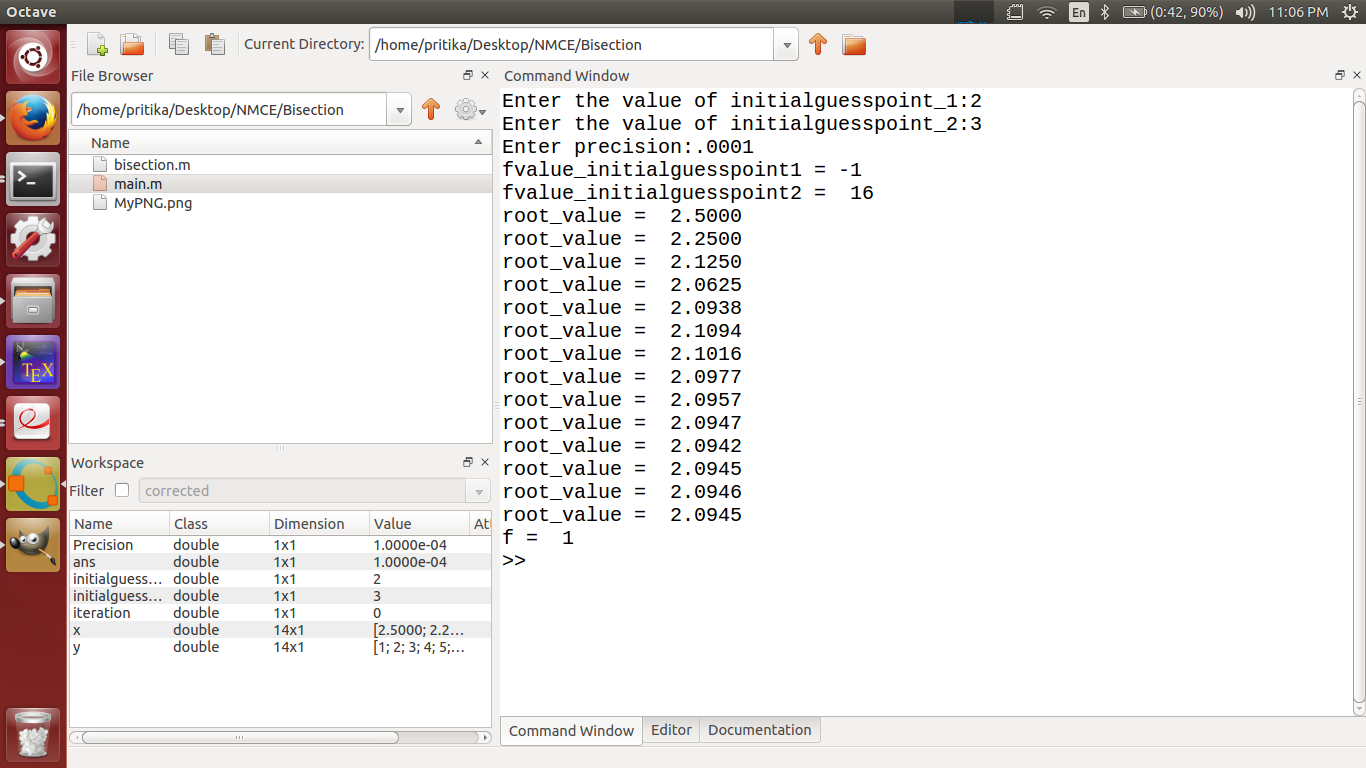
\includegraphics[width=0.7\textwidth]{images/bisection.png}                
	\caption{Bisection Method}
	\hspace{-1.5em}
\end{figure}\\

\textnormal After the user gets the approximate value, he final gets a plot which is saved in the same folder with name MYPNG.png as seen from Figure 4.2\\

\begin{figure}[!ht]
	\centering
	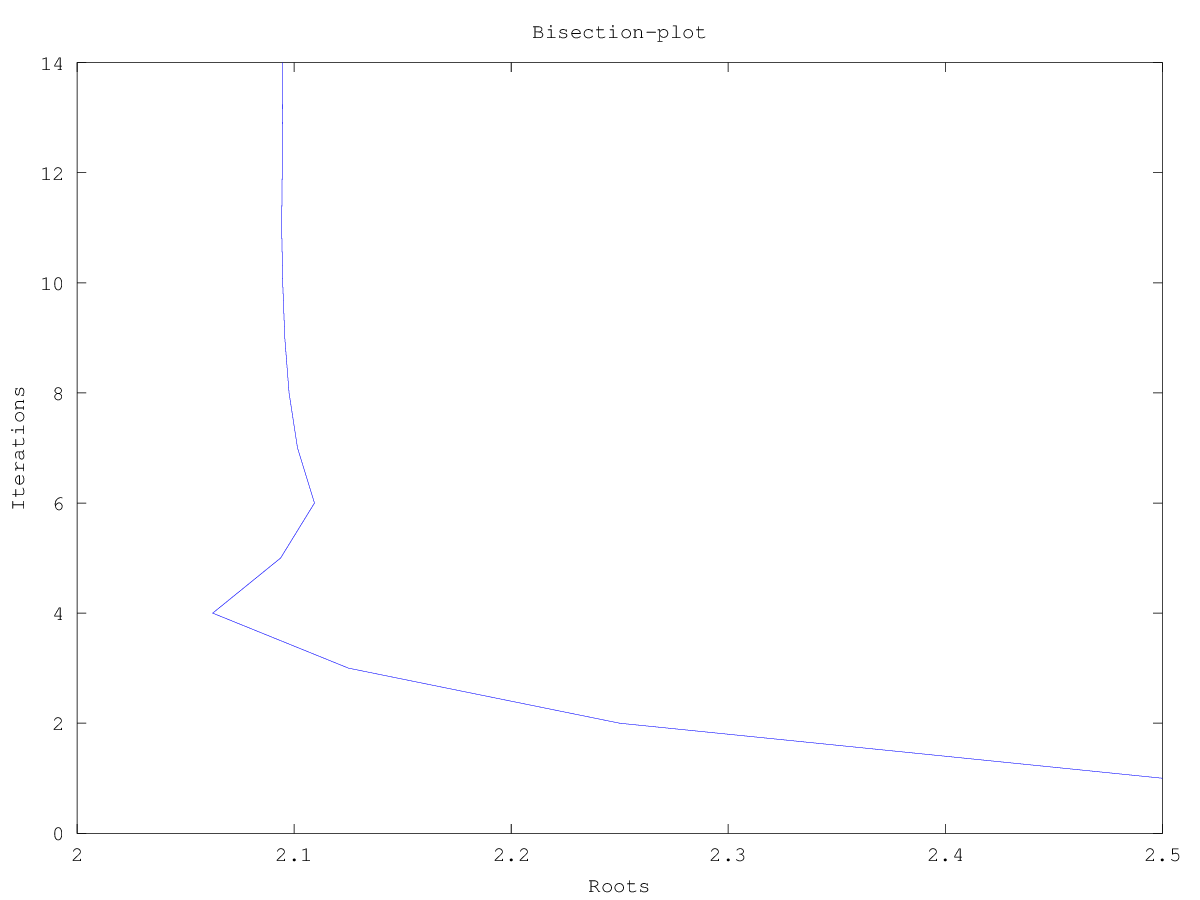
\includegraphics[width=0.7\textwidth]{images/mypng.png}                
	\caption{Bisection method plot}
	\hspace{-1.5em}
\end{figure}
\newpage
\textnormal Similarly in Euler's method, main method calls euler method.
User inputs initial values of x and y and step-size and the final value of x at which y is to be calculated.\\

Th plot can be seen by Figure 4.4\\
\begin{figure}[!ht]
	\centering
	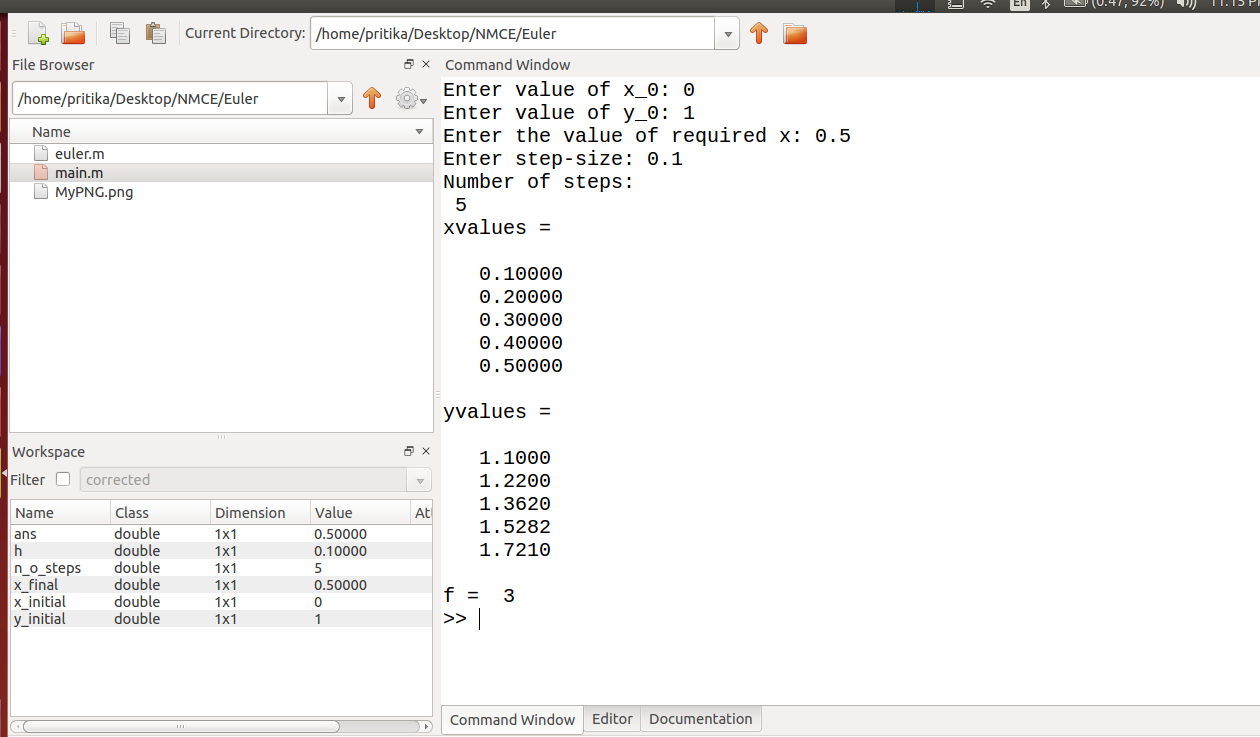
\includegraphics[width=0.7\textwidth]{images/euler.png}                
	\caption{Euler's Method}
	\hspace{-1.5em}
\end{figure}
User can find the plot saved in the same folder with name myeuler.png.
\begin{figure}[!ht]
	\centering
	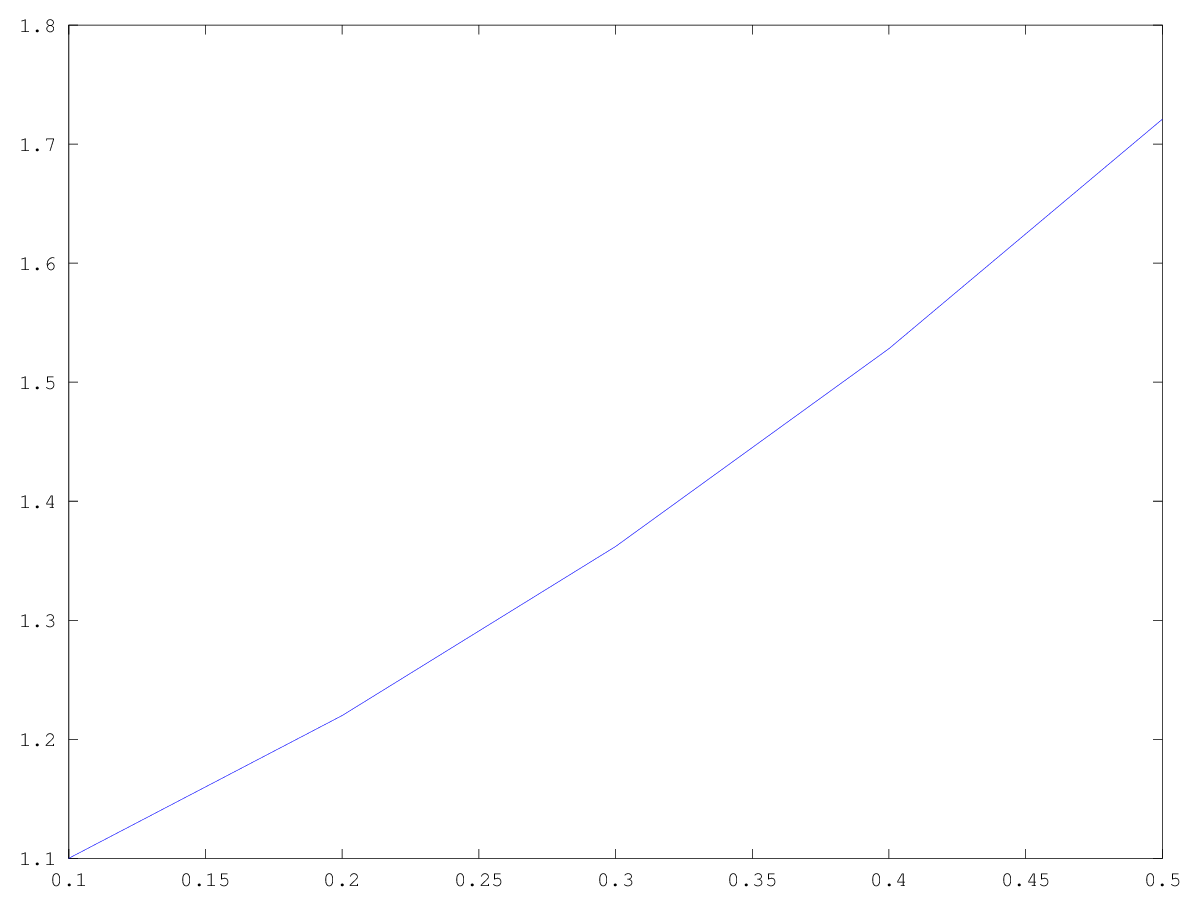
\includegraphics[width=0.7\textwidth]{images/myeuler.png}                
	\caption{Euler's method plot }
	\hspace{-1.5em}
\end{figure}
\newpage
 For methods dealing with matrices like,
 \textbf{Gauss Jordan}
 the user inputs the augmented matrix in the file and get the results:\\
 \begin{figure}[!ht]
 	\centering
 	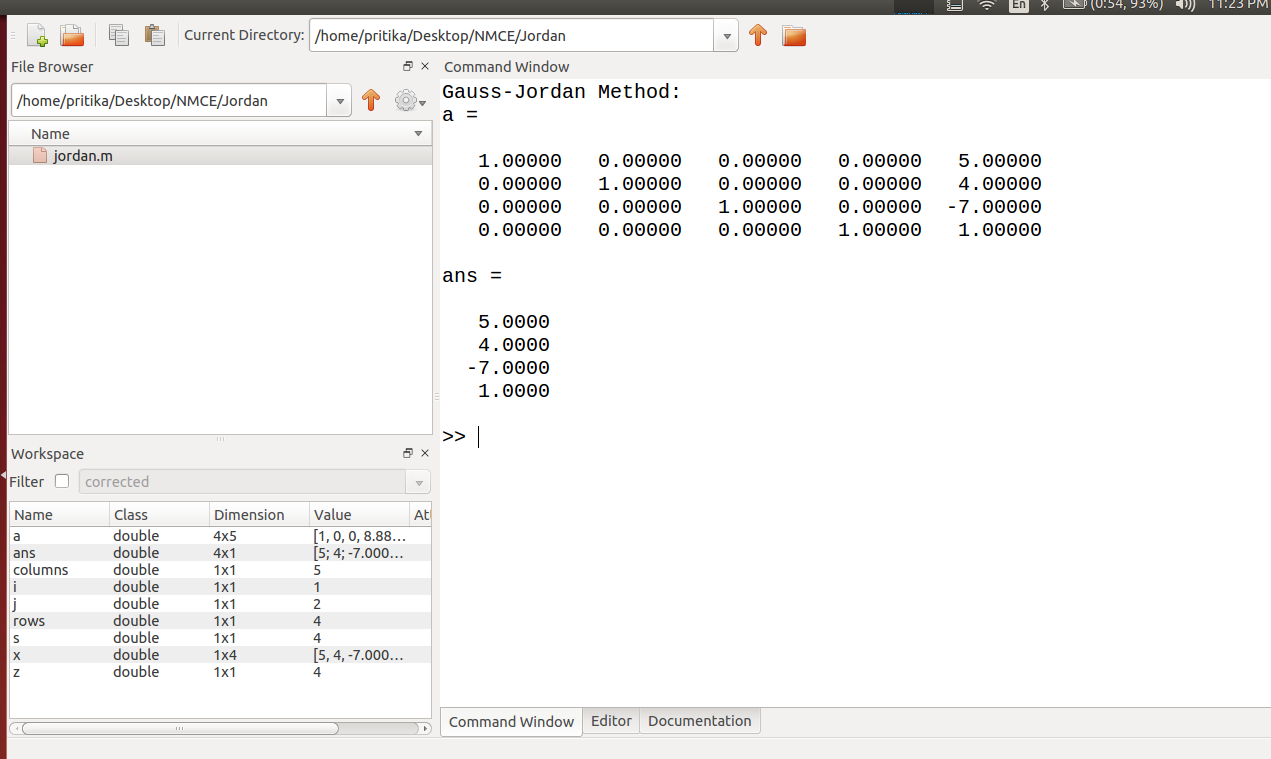
\includegraphics[width=0.7\textwidth]{images/jordan.png}                
 	\caption{Jordan method }
 	\hspace{-1.5em}
 \end{figure}
 \textbf{Gauss Elimination}
 The result for input matrix:\\
  \begin{figure}[!ht]
  	\centering
  	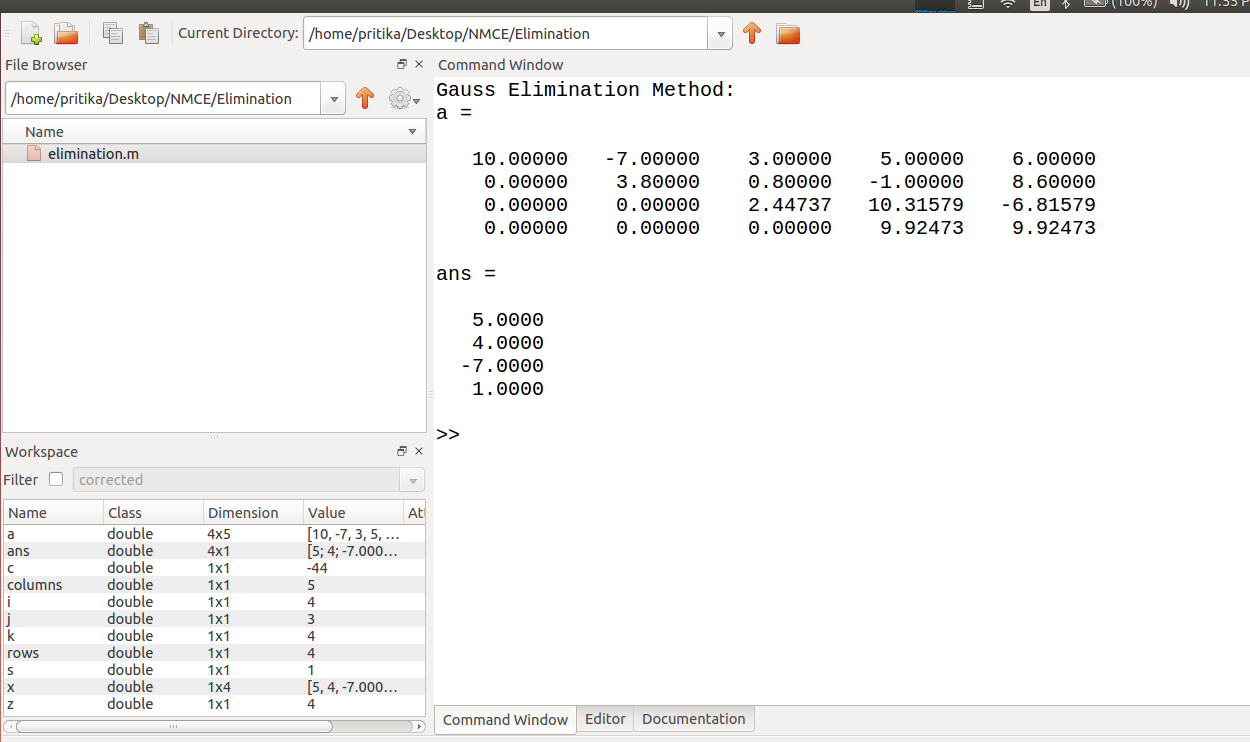
\includegraphics[width=0.7\textwidth]{images/Elimination.png}                
  	\caption{Elimination method }
  	\hspace{-1.5em}
  \end{figure}
  
  \newpage
  Weboctave is a web interface to octave:\\
  \begin{figure}[!ht]
  	\centering
  	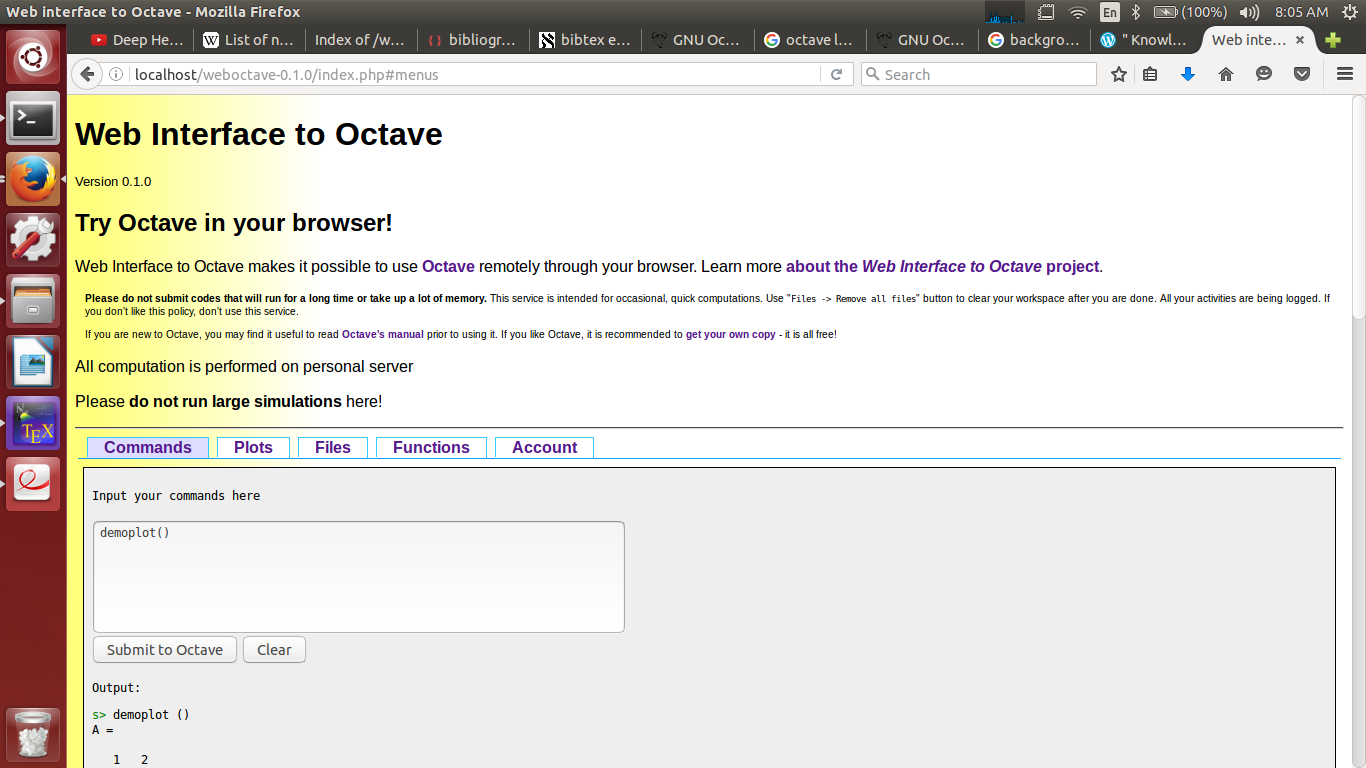
\includegraphics[width=0.7\textwidth]{images/interface.png}                
  	\caption{Weboctave Interface}
  	\hspace{-1.5em}
  \end{figure}
  

\noindent \textbf { The first query with which a user is greeted is:}\\

\noindent function demoplot()\\
A = [1,2;3,4]\\
eig(A)\\
y = x = linspace(0,10);
[X,Y] = meshgrid(x,y);\\
mesh(X,Y,sin(X).*cos(Y).*X);\\
endfunction\\

And it's result can be seen by: 

 \begin{figure}[!ht]
 	\centering
 	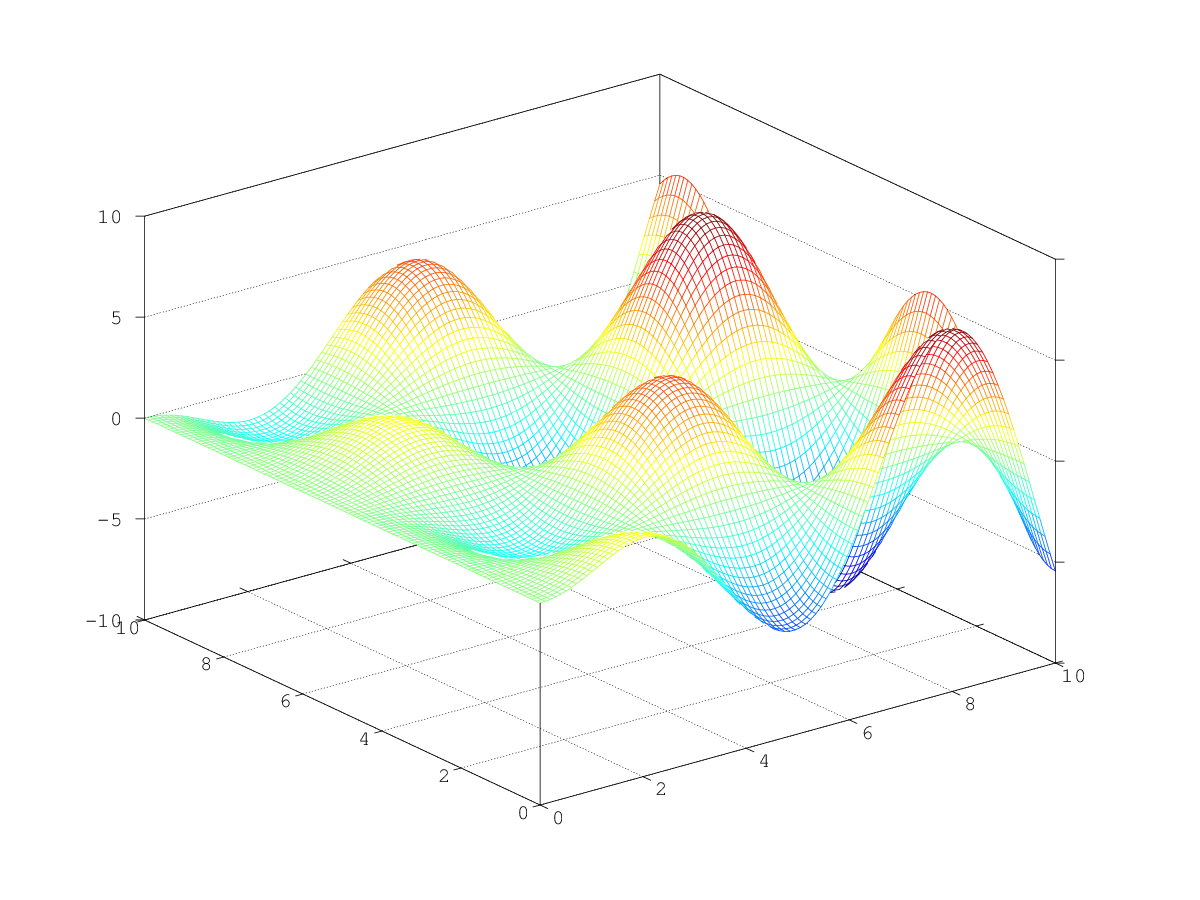
\includegraphics[width=0.7\textwidth]{images/plot1.png}                
 	\caption{Mesh}
 	\hspace{-1.5em}
 \end{figure}
 
 The plots obtained can be downloaded:\\
 \begin{figure}[!ht]
 	\centering
 	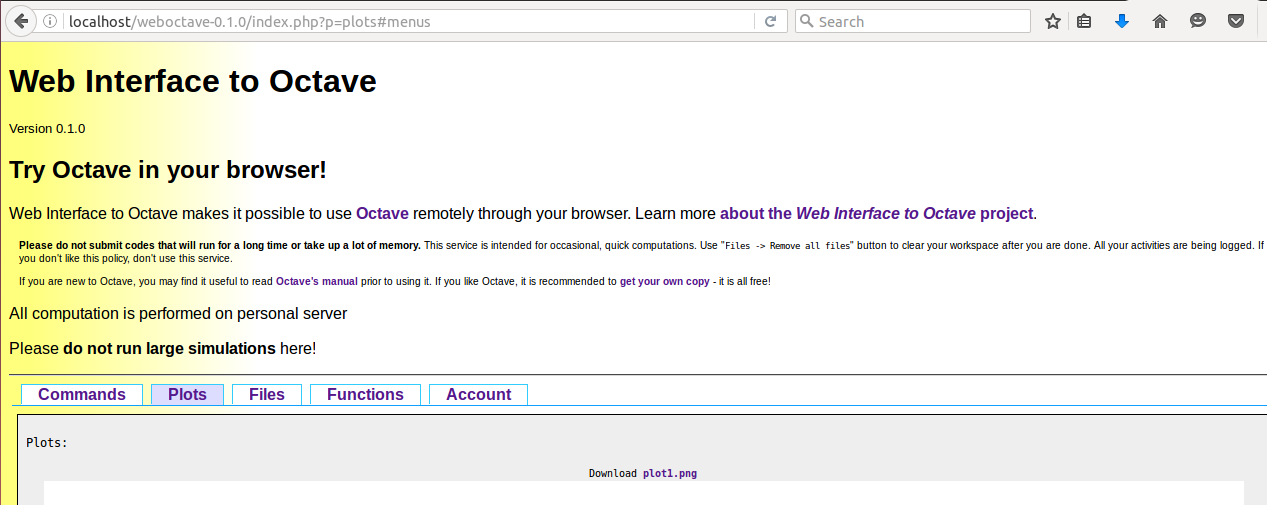
\includegraphics[width=0.7\textwidth]{images/download.png}                
 	\caption{Web Interface}
 	\hspace{-1.5em}
 \end{figure}
 \newpage
 User can create his/her account:
 \begin{figure}[!ht]
 	\centering
 	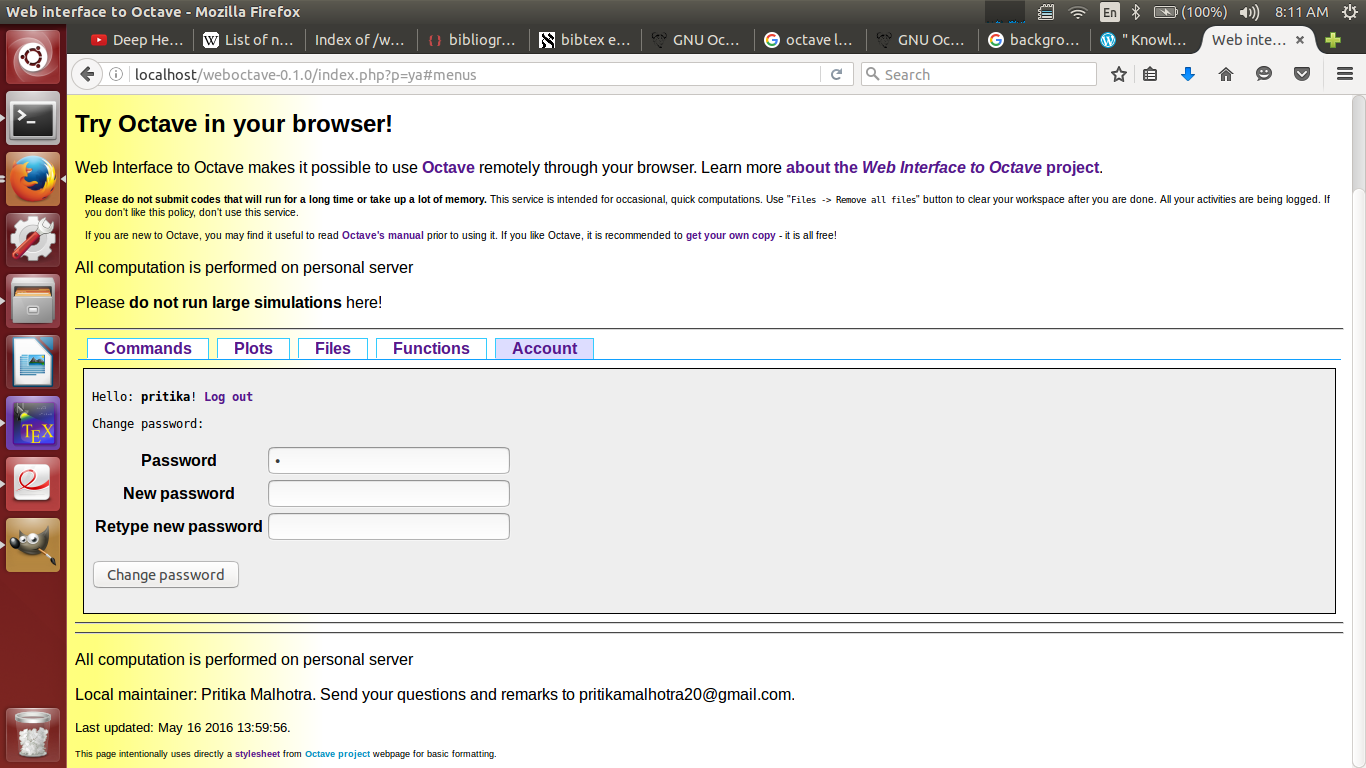
\includegraphics[width=0.7\textwidth]{images/account.png}                
 	\caption{User Accounts}
 	\hspace{-1.5em}
 \end{figure}
 
 
 
 
 